\section{Основы краудсорсинга для совместной экономики}

\textbf{Разъём TRS} (аббревиатура от англ. Tip, Ring, Sleeve — кончик, кольцо, гильза; подразумевается форма контактов на штекере) — распространённый разъём для передачи аудиосигнала. \cite{wiki-trs}

Однако, наверное мало кто из тех, кто сталкивался с этими разъемами в быту слышал, что они называются TRS, а все потому что у нас прижилось другое название. Его часто называют просто <<джек>>, и это никак не связано с какой-нибудь личностью по имени Джек: на самом деле с английского языка слово <<jack>> переводится как <<гнездо>>. Причем джеком правильно называть именно гнездо, то есть куда подключается, а это разъём-мама на панели, то есть на системном блоке или другом устройстве, а разъем-папу называют plug, что и переводится как <<штекер>>. \cite{kkg-jack}

\textbf{Джек (jack)} - это разъем диаметром 1/4 дюйма (6,3 мм). Применяется в музыкальном оборудовании, чаще всего Вы с ними встретитесь при использовании:
\begin{enumerate}
\item микрофонов для любителей (чаще всего это караоке или для домашней записи)
\item электрогитар, бас-гитар, педалей (<<примочек>>), усилителей для гитары.
\item профессиональных наушников
\item профессиональных звуковых плат
\end{enumerate}

\textbf{Мини-джек (mini-jack)} - разъём диаметром 3,5 мм. По сравнению с джеком действительно <<мини>>, и используется в устройствах, где размер действительно важен. Его вы можете встретить, купив:
\begin{enumerate}
\item наушники (обычные наушники для плеера, к примеру)
\item компьютерную акустичекую систему (её называют динамики или же колонки) 
\item гарнитуру
\item плеер
\item звуковую плату потребительского уровня
\end{enumerate}

\begin{figure}[h]
  \centering
  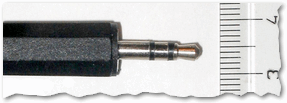
\includegraphics[scale=1]{mini-jack-audio.png}
  \caption{Разъем мини-jack}
  \label{image:mini-jack-audio}
\end{figure}

\begin{figure}[h]
  \centering
  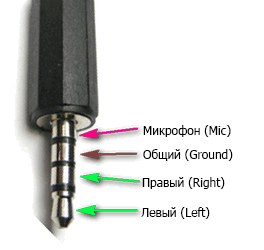
\includegraphics[scale=1]{headset.png}
  \caption{Гарнитурный штекер}
  \label{image:headset}
\end{figure}

На ноутбуках есть два вида разъемов, предназначеных для подключения акустической системы и микрофона. Они показаны на Рисунке ~\ref{image:notebook}. Для подключения гарнитуры с стандартным совмещенным штекером (Рисунок ~\ref{image:headset}) в левый разъем (Рисунок ~\ref{image:notebook}) используется переходник, показанный на рисунке ~\ref{image:adapter}.

\begin{figure}[h]
  \centering
  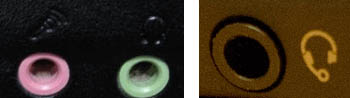
\includegraphics[scale=1]{notebook.jpg}
  \caption{Разъемы ноутбука}
  \label{image:notebook}
\end{figure}

\begin{figure}[h]
  \centering
  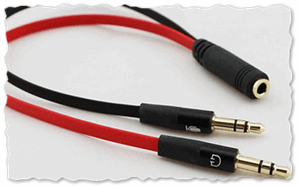
\includegraphics[scale=1]{adapter.png}
  \caption{Переходник для подключения гарнитурных наушников к обычной звуковой карте}
  \label{image:adapter}
\end{figure}

\section{Звуковая архитектура}

Рисунок \ref{image:sound_arch} показывает подключение звука на ПК-совместимой системе. Аудио контроллер Южного моста, а также внешний кодек, подключённый к аналоговой звуковой схеме. \cite{eldd}

\begin{figure}[h]
  \centering
  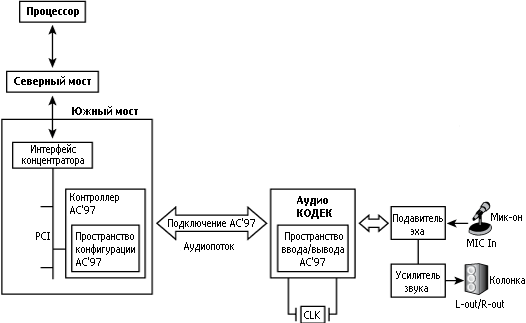
\includegraphics[scale=0.8]{sound_arch.png}
  \caption{Звук в среде ПК}
  \label{image:sound_arch}
\end{figure}

\subsection{Звуковая подсистема Linux}

\subsection{Open Sound System}
\textbf{Open Sound System} (OSS) — унифицированный драйвер для звуковых карт и других звуковых устройств в различных UNIX-подобных операционных системах.

OSS основан на Linux Sound Driver и в настоящее время работает на большом числе платформ: Linux, FreeBSD, OpenSolaris и т. д. \cite{wiki-oss}

/dev/dsp и /dev/audio — основные файлы устройств для цифровых приложений. Любые данные, записанные в эти файлы, воспроизводятся на DAC/PCM/DSP устройстве звуковой карты. Чтение из этих файлов возвращает звуковые данные, записанные с текущего входного источника (по умолчанию это Микрофонный вход).

При чтении из /dev/dsp мы получаем несжатый аудиопоток с микрофона компьютера через вход звуковой карты. 

\subsection{ALSA}

\textbf{ALSA} (англ. Advanced Linux Sound Architecture, Продвинутая звуковая архитектура Linux) — архитектура звуковых драйверов, а также широкий их набор для операционной системы Linux, призванный сменить Open Sound System (OSS). ALSA тесно связана с ядром Linux. ALSA — программный микшер, который эмулирует совместимость для других слоев. Также предоставляет API для программистов и работает с низкой стабильной задержкой. \cite{wiki-alsa}

ALSA является звуковой подсистемой, выбранной  для ядра версии 2.6. Открытая Звуковая Система, OSS, звуковой уровень в ядре версии 2.4, в настоящее время устарел и не рекомендуется к использованию. Для перехода от OSS к ALSA последняя предоставляет эмуляцию OSS, которая позволяет приложениям, использующим API OSS, запускаться без изменений на ALSA. Звуковые ядра Linux, такие как ALSA и OSS, делают аудио приложения независимыми от базового оборудования.

Чтобы понять архитектуру звуковой подсистемы Linux посмотрите на Рисунок  \ref{image:sound_system}. 

\begin{figure}[h]
  \centering
  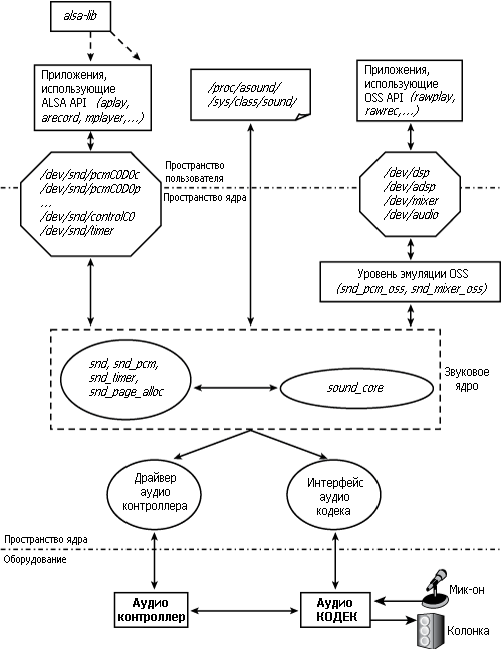
\includegraphics[scale=0.8]{sound_system.png}
  \caption{Звуковая подсистема Linux (ALSA)}
  \label{image:sound_system}
\end{figure}

Основными частями подсистемы являются:

\begin{enumerate}
\item Звуковое ядро, которое является базовым кодом, состоящим из процедур и структур, доступных другим компонентам звукового уровня Linux. Как и уровни ядра, принадлежащие другим драйверным подсистемам, звуковое ядро обеспечивает уровень косвенности, что делает каждый компонент в звуковой подсистеме не зависящим от других. Ядро играет важную роль в экспорте API ALSA вышележащим приложениям. Узлами /dev/snd/*, показанными на Рисунке \ref{image:sound_system}, которые создаются и управляются из ядром ALSA, являются: /dev/snd/controlC0 - узел управления (используемый в приложениях для управления уровнем громкости и тому подобному), /dev/snd/pcmC0D0p - устройство воспроизведения (p в конце имени устройства означает playback, воспроизведение), и /dev/snd/pcmC0D0c - записывающее устройство (c в конце имени устройства означает capture, захват). В этих именах устройств целое число после C является номером карты, а после D - номером устройства. ALSA драйвер для карты, которая имеет голосовой кодек для телефонии и стерео кодек для музыки, может экспортировать /dev/snd/pcmC0D0p для чтения аудио потоков, предназначенный для первого, и /dev/snd/pcmC0D1p для качественного музыкального канала для последнего.
 
\item Драйверы аудио контроллера зависят от оборудования контроллера. Например, для управления аудио контроллером, находящимся в Южном мосте Intel ICH, используется драйвер snd\_intel8x0.
 
\item Интерфейсы аудиокодеков, которые помогают взаимодействию между контроллерами и кодеками. Для кодеков AC'97 используйте snd\_ac97\_codec и модули ac97\_bus.
 
\item Уровень эмуляции OSS, который выступает в качестве посредника между приложениями, использующими OSS, и ядром с поддерживающим ALSA. Этот уровень экспортирует узлы /dev, изображающие поддержку уровня OSS в ядре версии 2.4. Эти узлы, такие как /dev/dsp, /dev/adsp и /dev/mixer, позволяют приложениям OSS работать поверх ALSA без изменений. Узел OSS /dev/dsp связан с узлами ALSA /dev/snd/pcmC0D0*, /dev/adsp соответствует /dev/snd/pcmC0D1*, а /dev/mixer связан с /dev/snd/controlC0.
 
\item Интерфейс procfs and sysfs для доступа к информации через /proc/asound/ и /sys/class/sound/.
 
\item Библиотека ALSA пользовательского пространства, alsa-lib, которая предоставляет объект libasound.so. Эта библиотека упрощает работу программиста приложения ALSA, предлагая несколько готовых процедур для доступа к драйверам ALSA.

\item Пакет alsa-utils, который включает в себя такие утилиты, как alsamixer, amixer, alsactl и aplay. alsamixer или mixer используются для изменения громкости звуковых сигналов, таких как линейный вход, линейный выход или микрофон, а alsactl - для управления параметрами драйверов ALSA. aplay используется для воспроизведения звука через ALSA.
\end{enumerate}

В данной работе для получения потока байтов от микрофонного разъема будем использовать API, предоставляемые ALSA.
